\chapter{Apresentação dos Resultados}

Nessa seção, apresentaremos os resultados obtidos através dos modelos preditivos ARIMA e LSTM para a previsão da temperatura do ano de 2019. 

A Figura \ref{fig:results_histogram_arima_model_rmse} apresenta um histograma de comparação entre o erro médio quadrático (RMSE) obtido em cada um dos modelos, ARIMA e LSTM, para a previsão da temperatura do ano de 2019 nas 88 estações avaliadas. Analisando o gráfico podemos afirmar que o modelo LSTM teve mais estações com os menores erros, abaixo de 1,5, enquanto que o modelo ARIMA apresentou mais estações com os maiores erros, acima de 2,0. Para todas as 88 estações avaliadas, o RMSE  Global, ou seja, a média de todos os erros, foi 2,67 para o modelo ARIMA e 1,38 para o modelo LSTM, indicando que o modelo LSTM teve um desempenho na previsão muito melhor que o modelo ARIMA. 
 
 \begin{figure}[H]
    \centering
    \caption{Comparação entre os valores obtidos de RMSE para as 88 estações avaliadas.}
    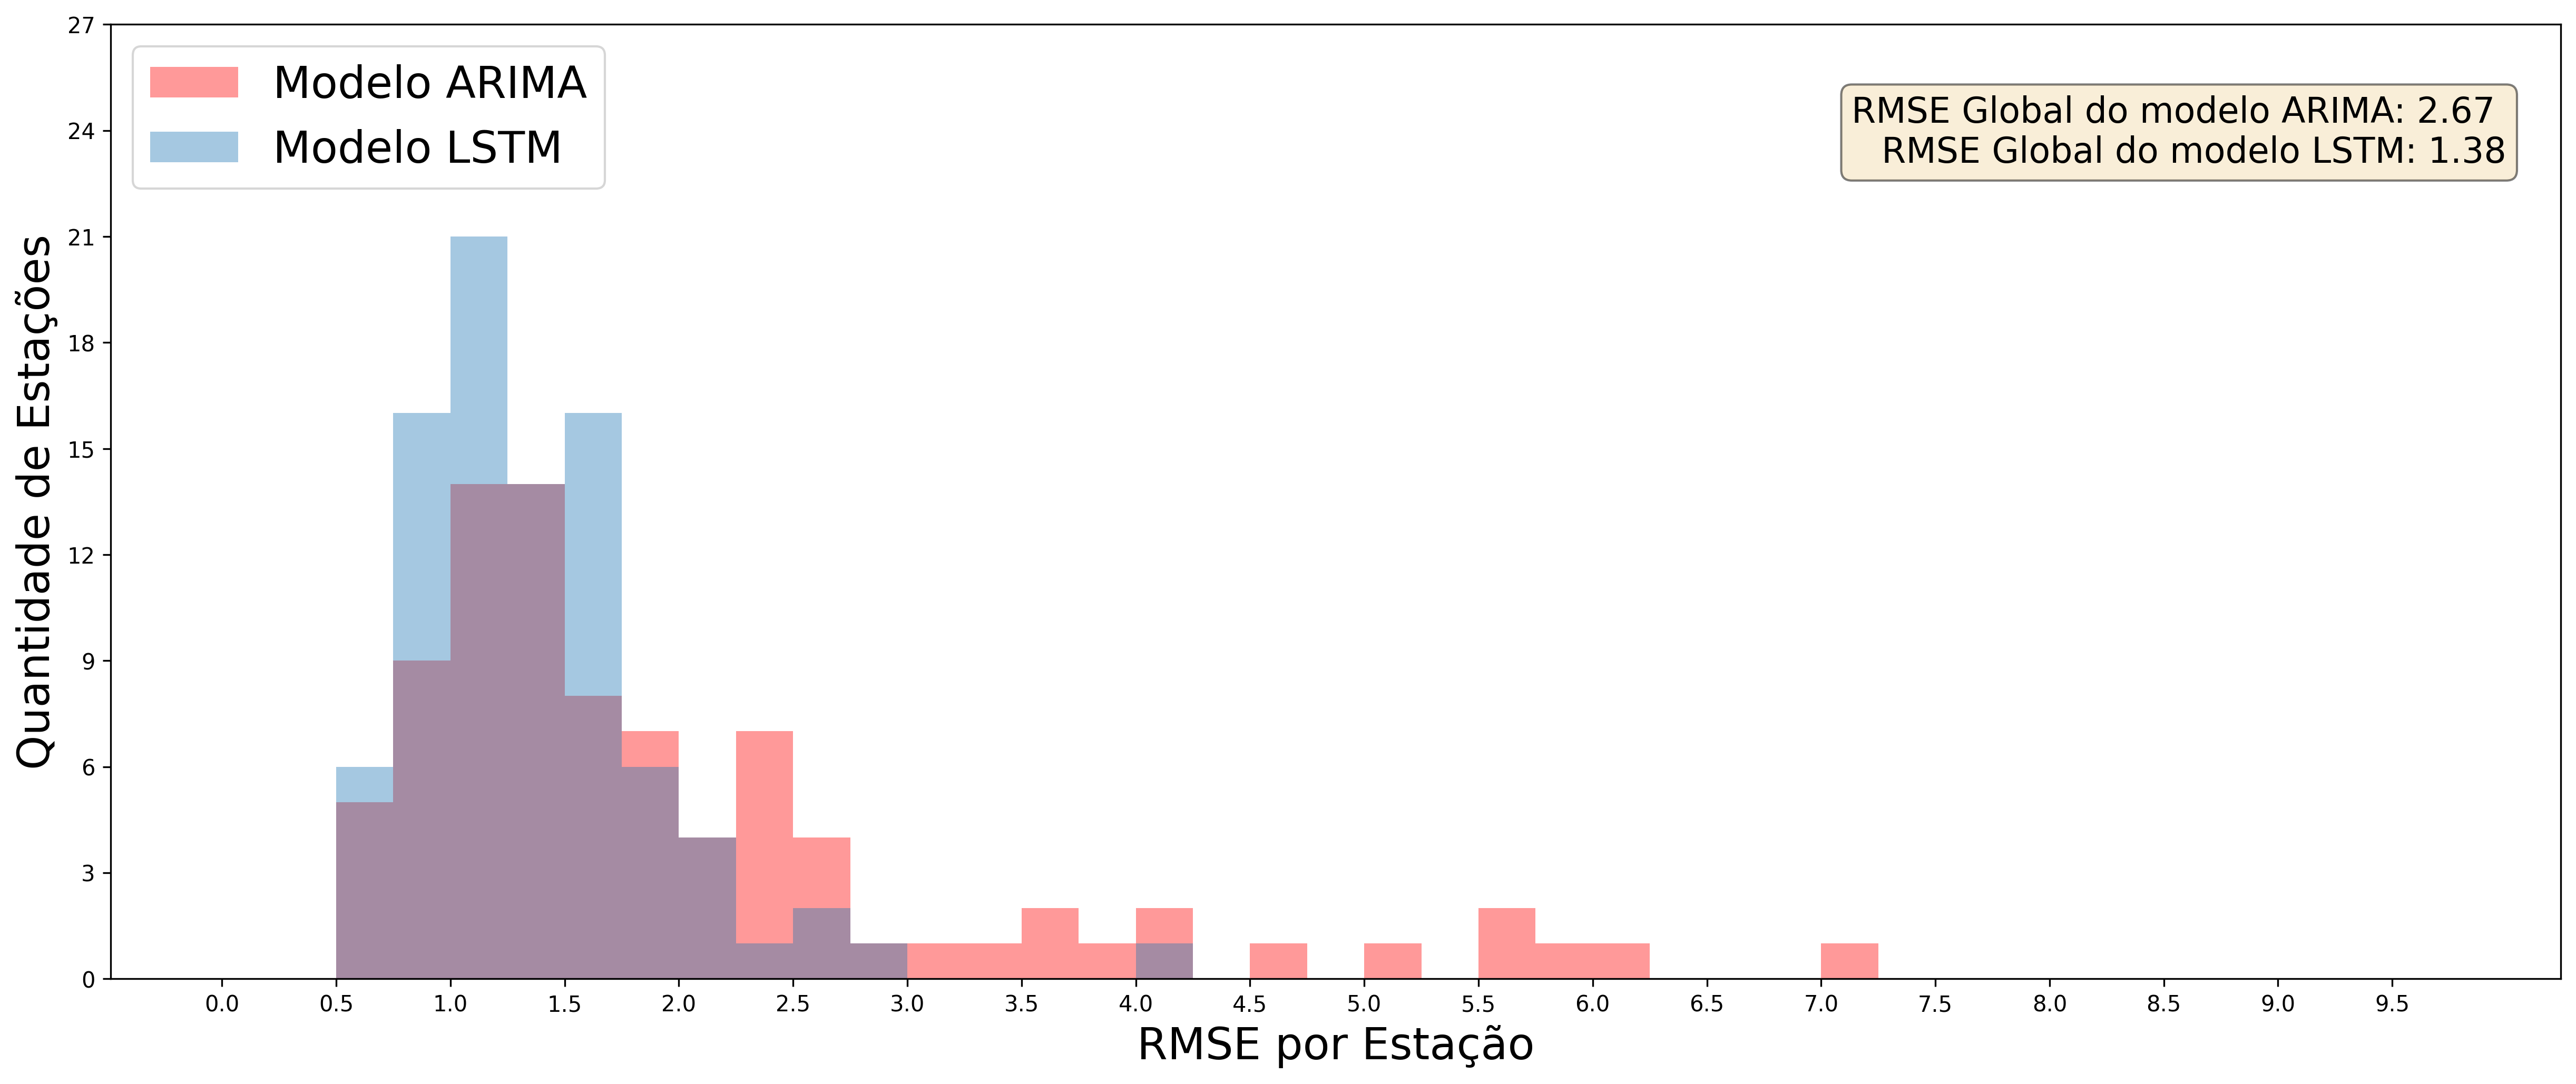
\includegraphics[width=\textwidth]{figuras/results/comparacao_rmse_arima_lstm_histograma.png}
    \label{fig:results_histogram_arima_model_rmse}
\end{figure}

Analisando as previsões individuais, ilustramos na Figura \ref{fig:results_arima_A826} o resultado da previsão para uma estação localizada no município de São Luiz Gonzaga, no estado do Rio Grande do Sul. Para essa estação em que o modelo ARIMA apresentou um maior erro, acima de 5, o modelo LSTM conseguiu uma boa performance alcançando um erro um pouco acima de 1,8. Esse comportamento se refletiu em diversas outras estações em que o modelo ARIMA teve um resultado pior em relação ao seu próprio RMSE Global.  

\begin{figure}[H]%
\caption{Resultado das previsões da temperatura do ar para o ano de 2019 da estação meteorológica localizada no município de São Luiz Gonzaga, no estado do Rio Grande do Sul.}
\centering
\subfloat{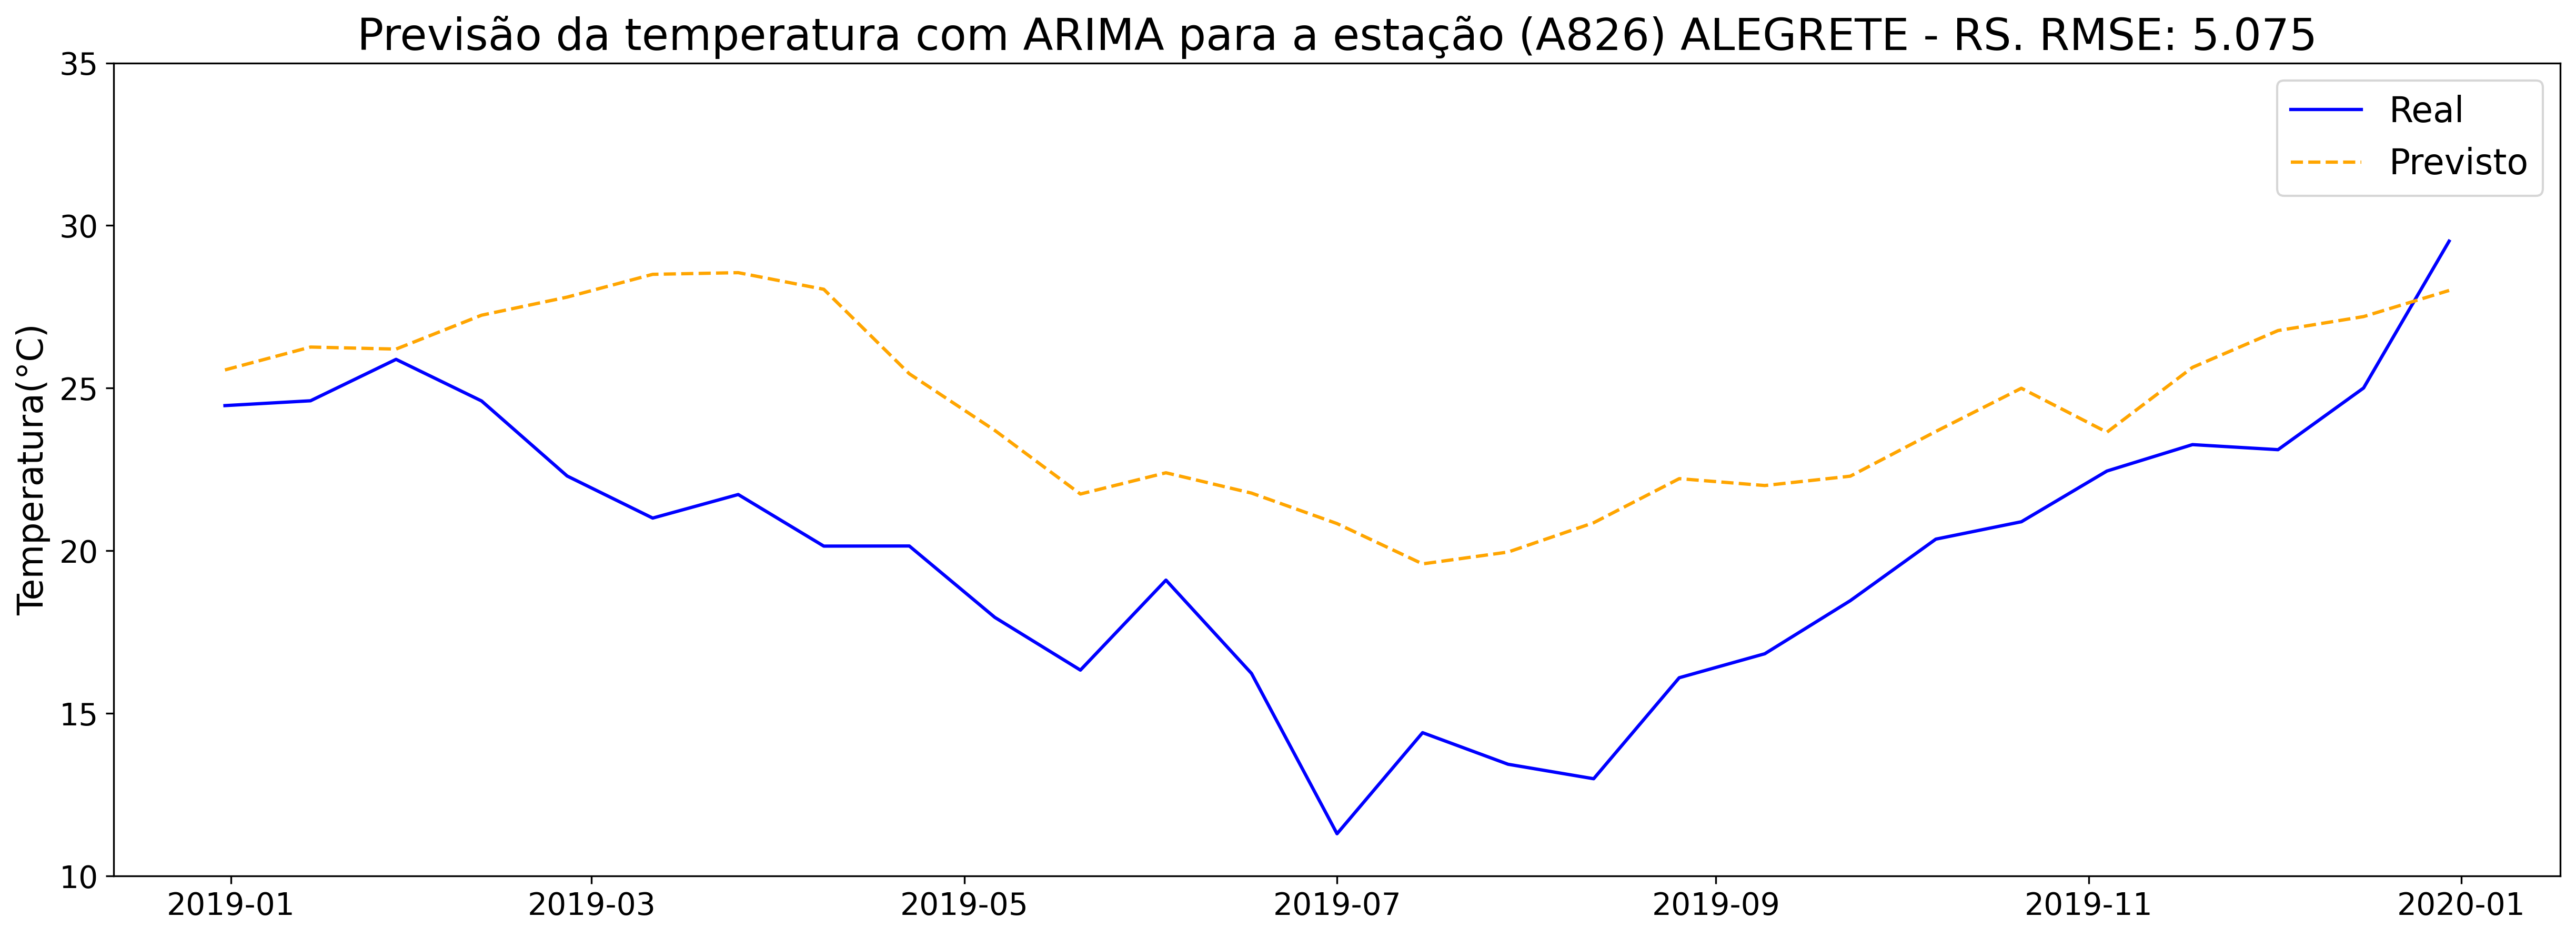
\includegraphics[scale=.30]{figuras/results/results_arima_A826.png}}
\qquad
\subfloat{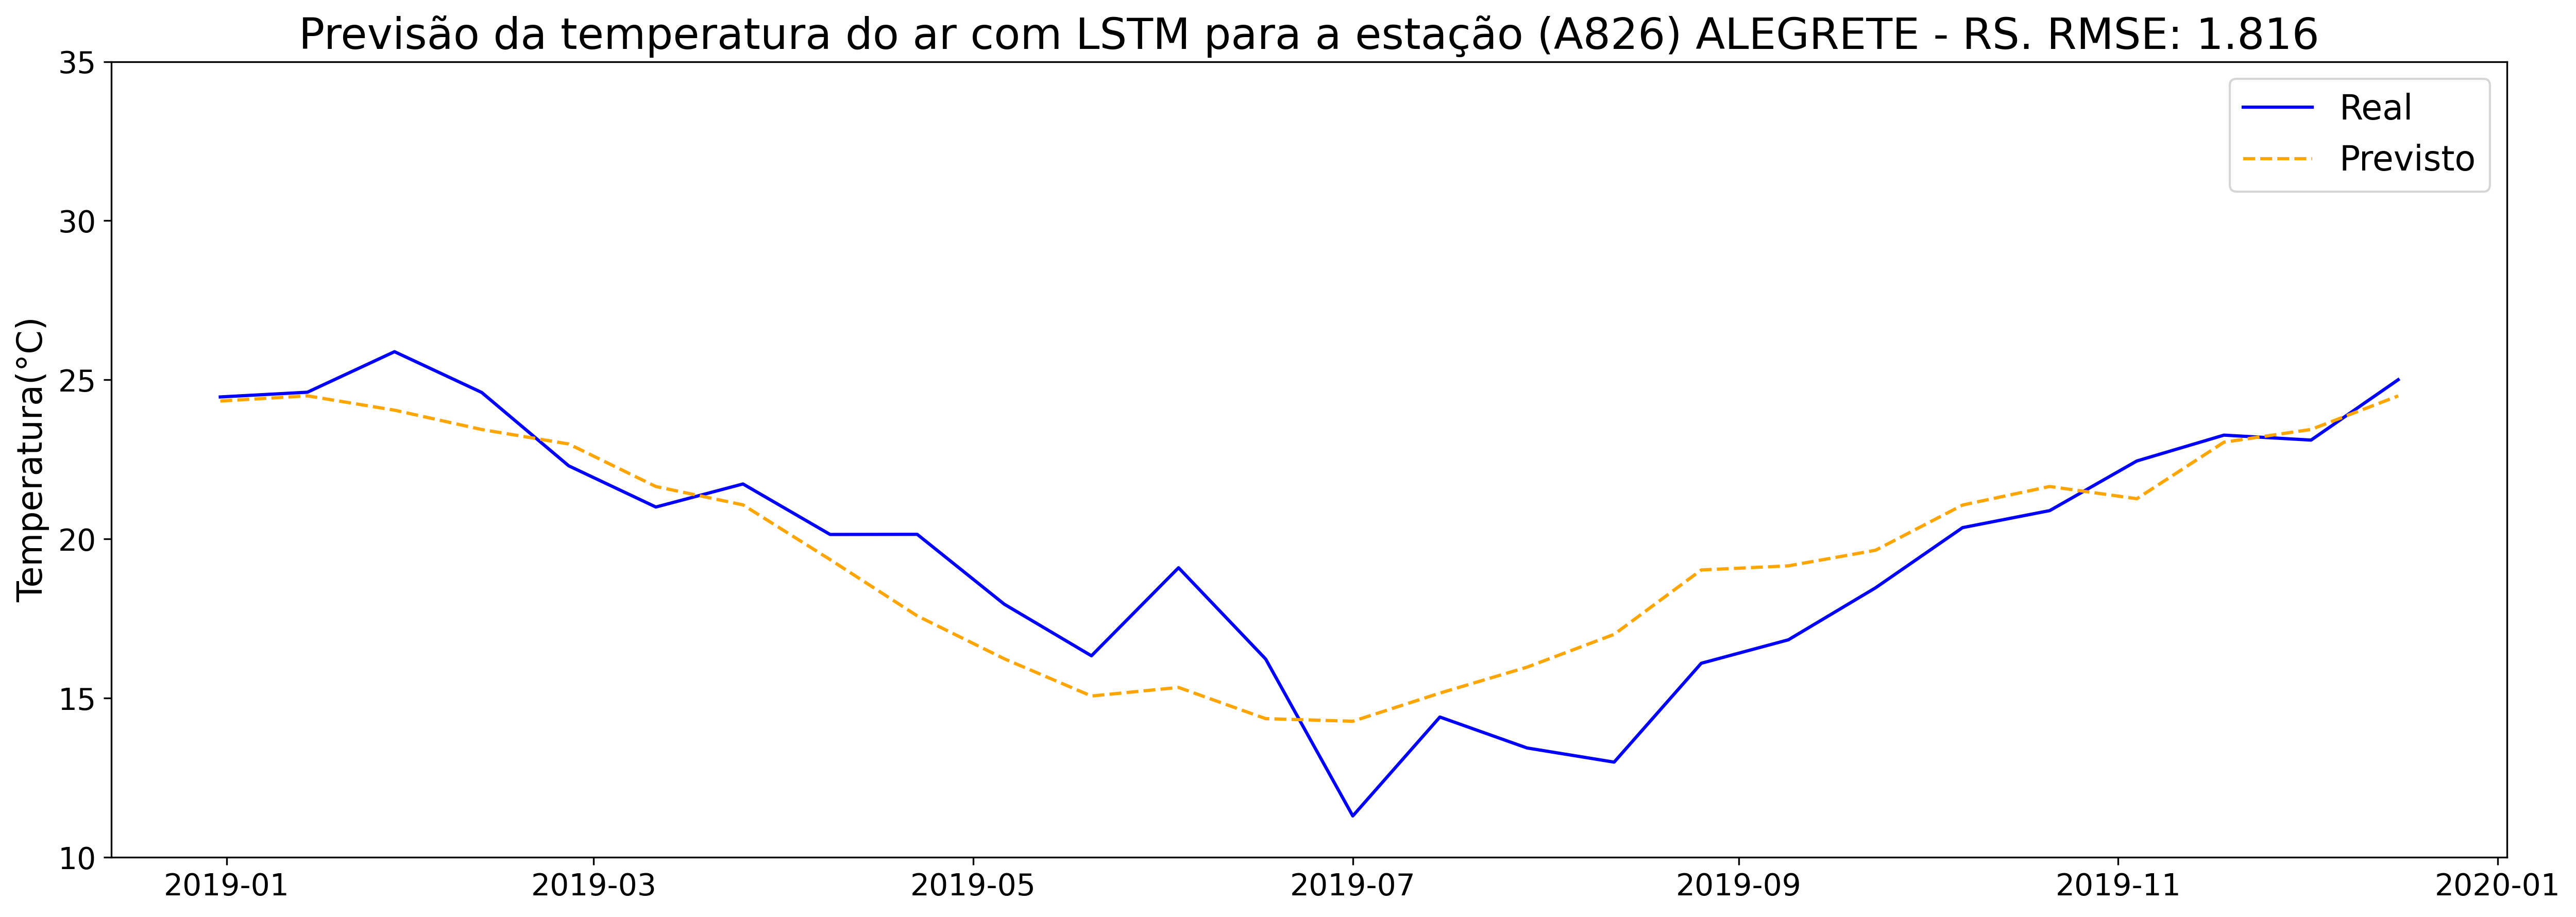
\includegraphics[scale=.30]{figuras/results/results_lstm_A826.png}}
\label{fig:results_arima_A826}%
\end{figure}

Avaliando as estações em que o modelo LSTM teve um desempenho pior do seu seu próprio RMSE Global, identificamos que, nessas estações, o modelo ARIMA não obteve grande vantagem, nas raras vezes em que foi melhor, em relação ao modelo LSTM. Na Figura \ref{fig:results_arima_A720} adicionamos um exemplo do resultado da previsão para uma estação em que o modelo LSTM não conseguiu bons resultados. Nas figuras \ref{fig:results_lstm_83464} e \ref{fig:results_lstm_83361} também apresentamos o resultados da previsão para outras estações. 

\begin{figure}[H]%
\caption{Resultado das previsões da temperatura do ar para o ano de 2019 da estação meteorológica localizada no município de São Luiz Gonzaga, no estado do Rio Grande do Sul.}
\centering
\subfloat{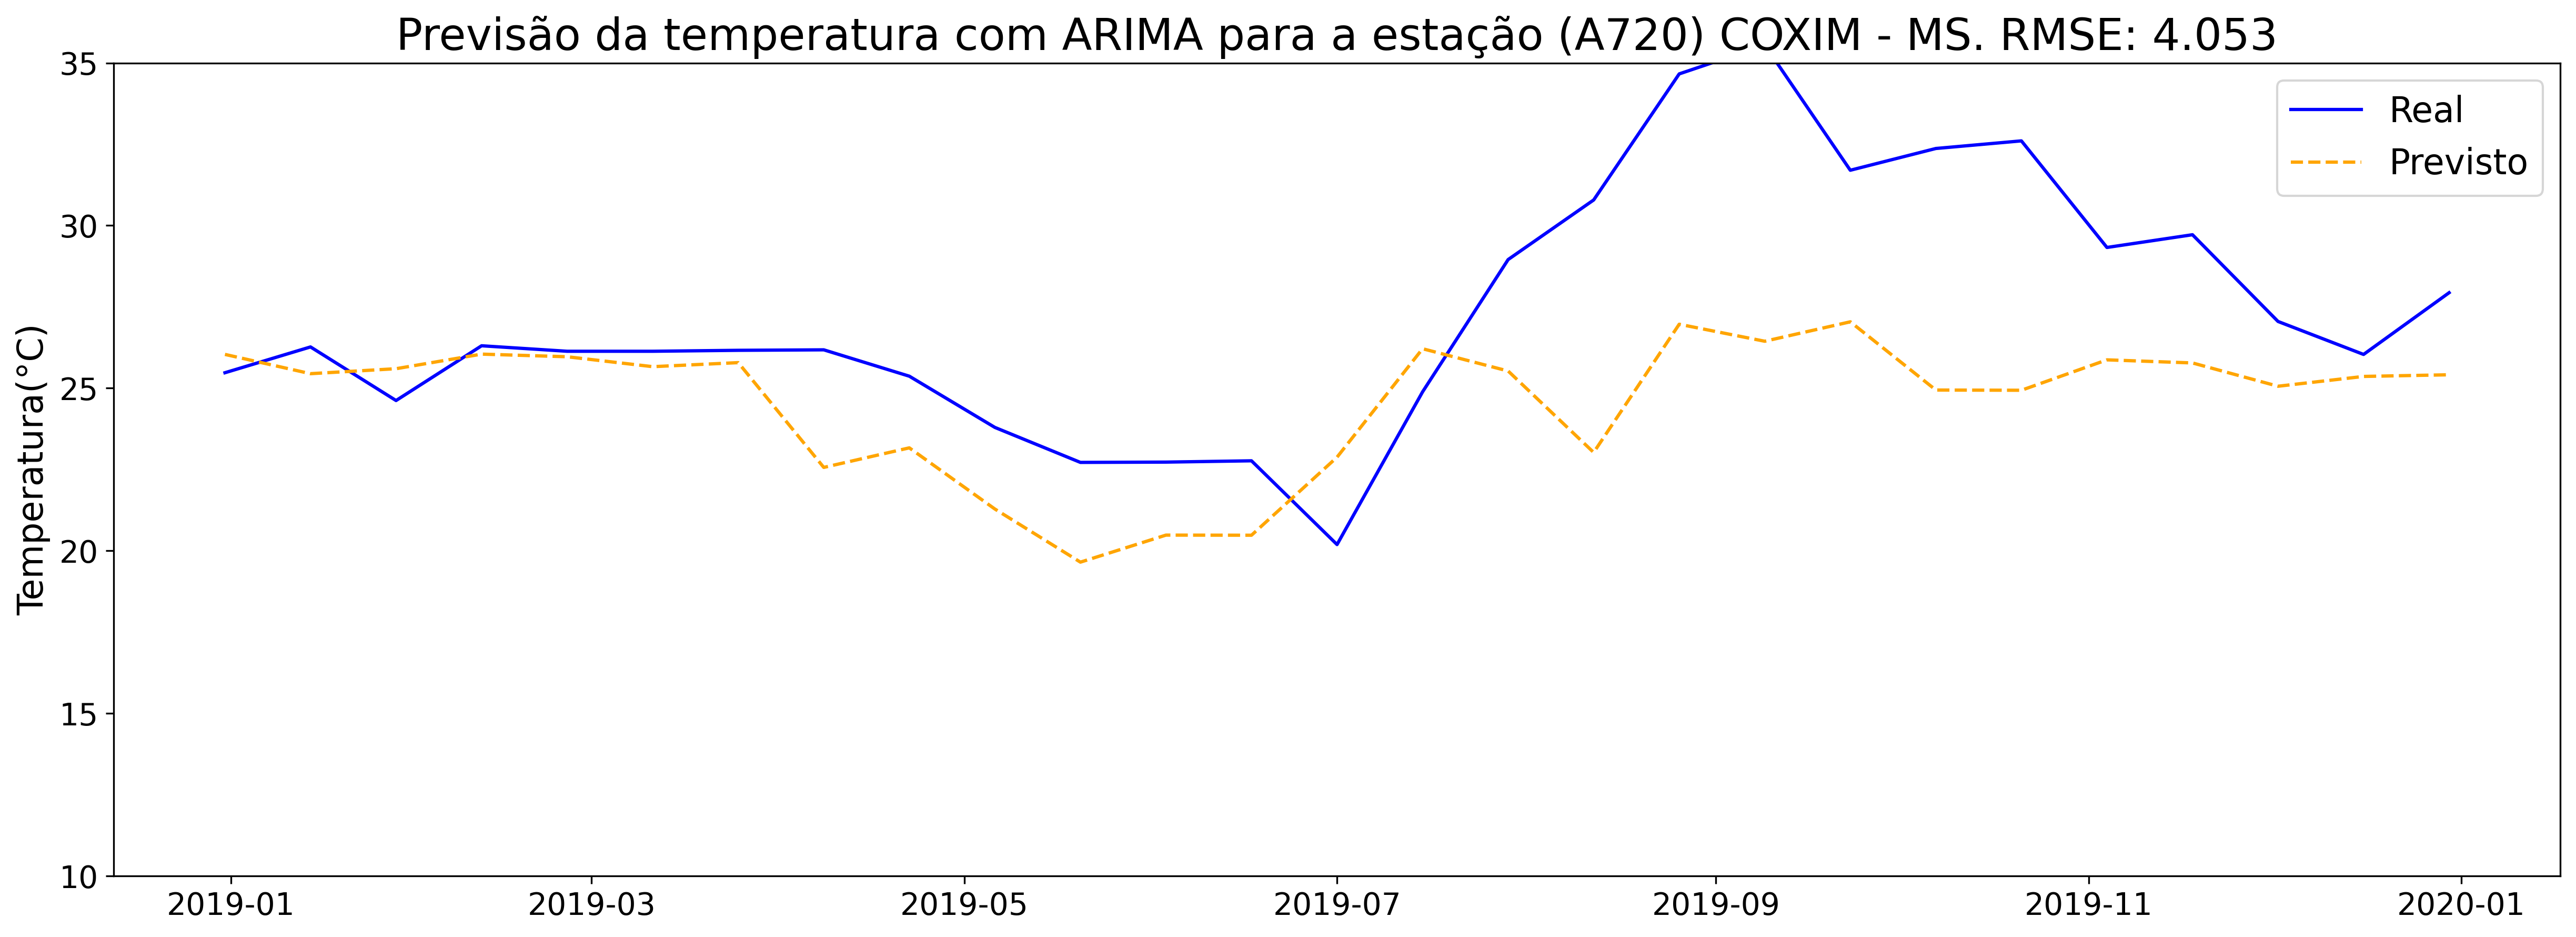
\includegraphics[scale=.30]{figuras/results/results_arima_A720.png}}
\qquad
\subfloat{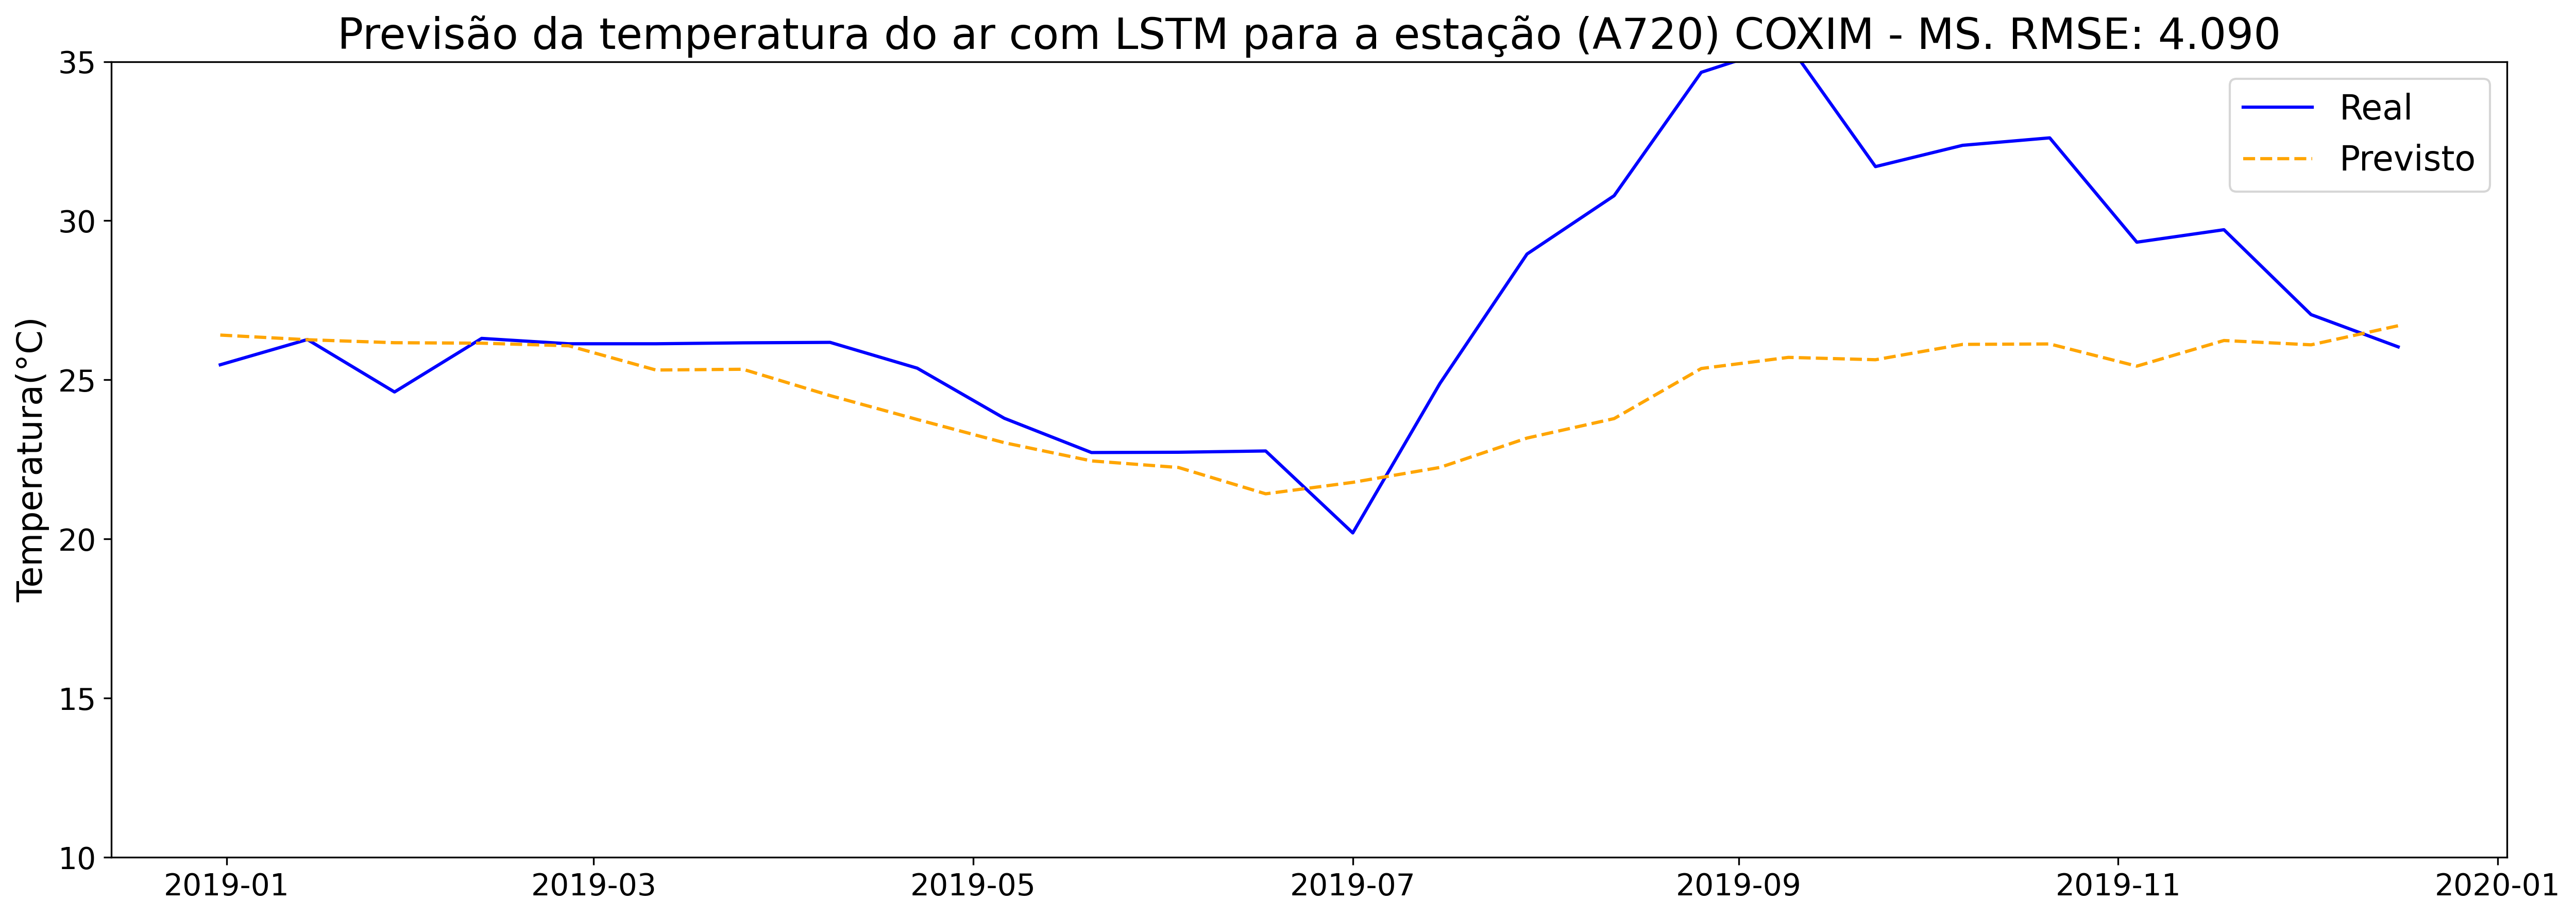
\includegraphics[scale=.30]{figuras/results/results_lstm_A720.png}}
\label{fig:results_arima_A720}%
\end{figure}

\begin{figure}[H]%
\caption{Resultado das previsões da temperatura do ar para o ano de 2019 da estação meteorológica localizada no município de São Luiz Gonzaga, no estado do Rio Grande do Sul.}
\centering
\subfloat{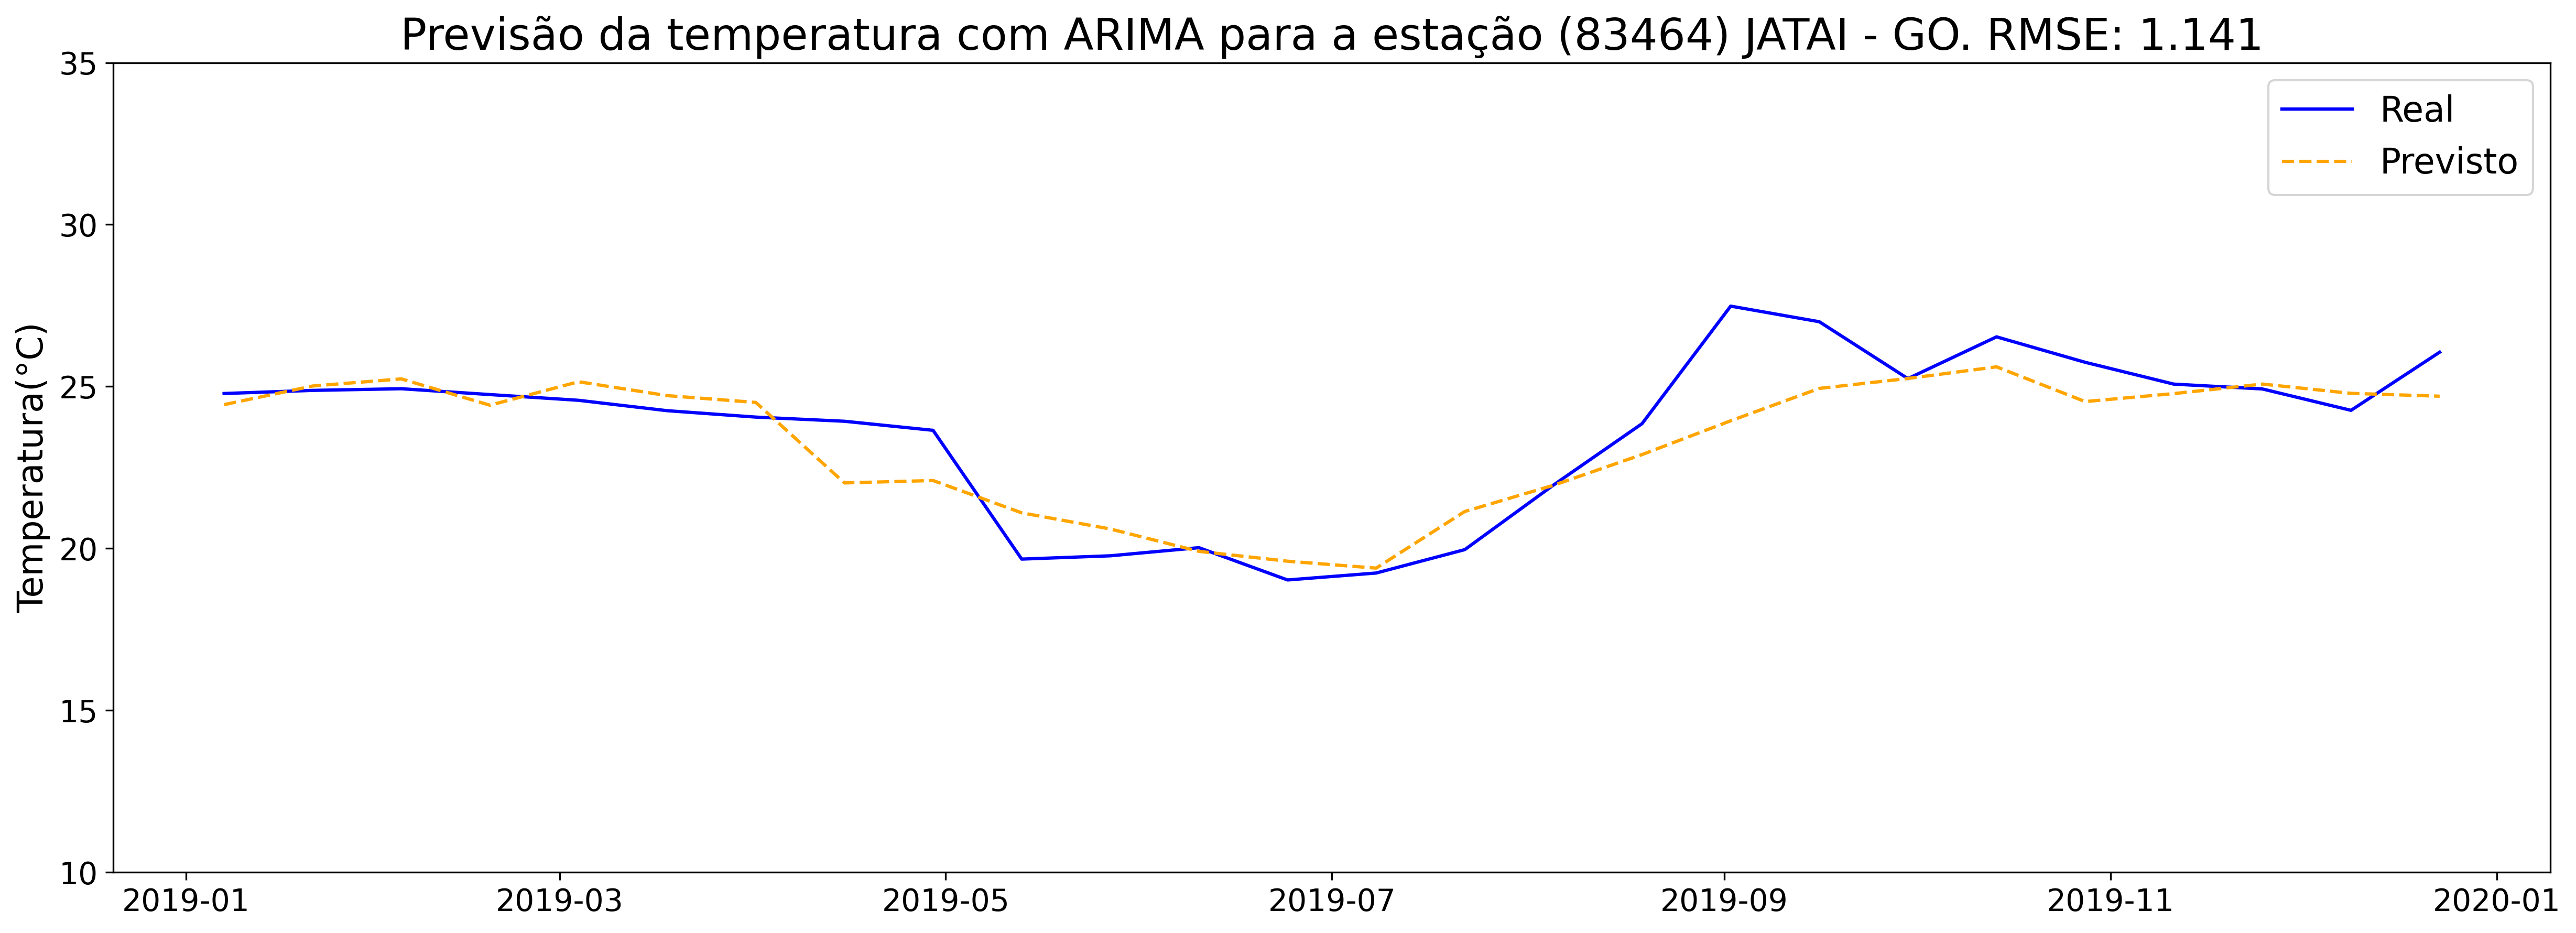
\includegraphics[scale=.30]{figuras/results/results_arima_83464.png}}
\qquad
\subfloat{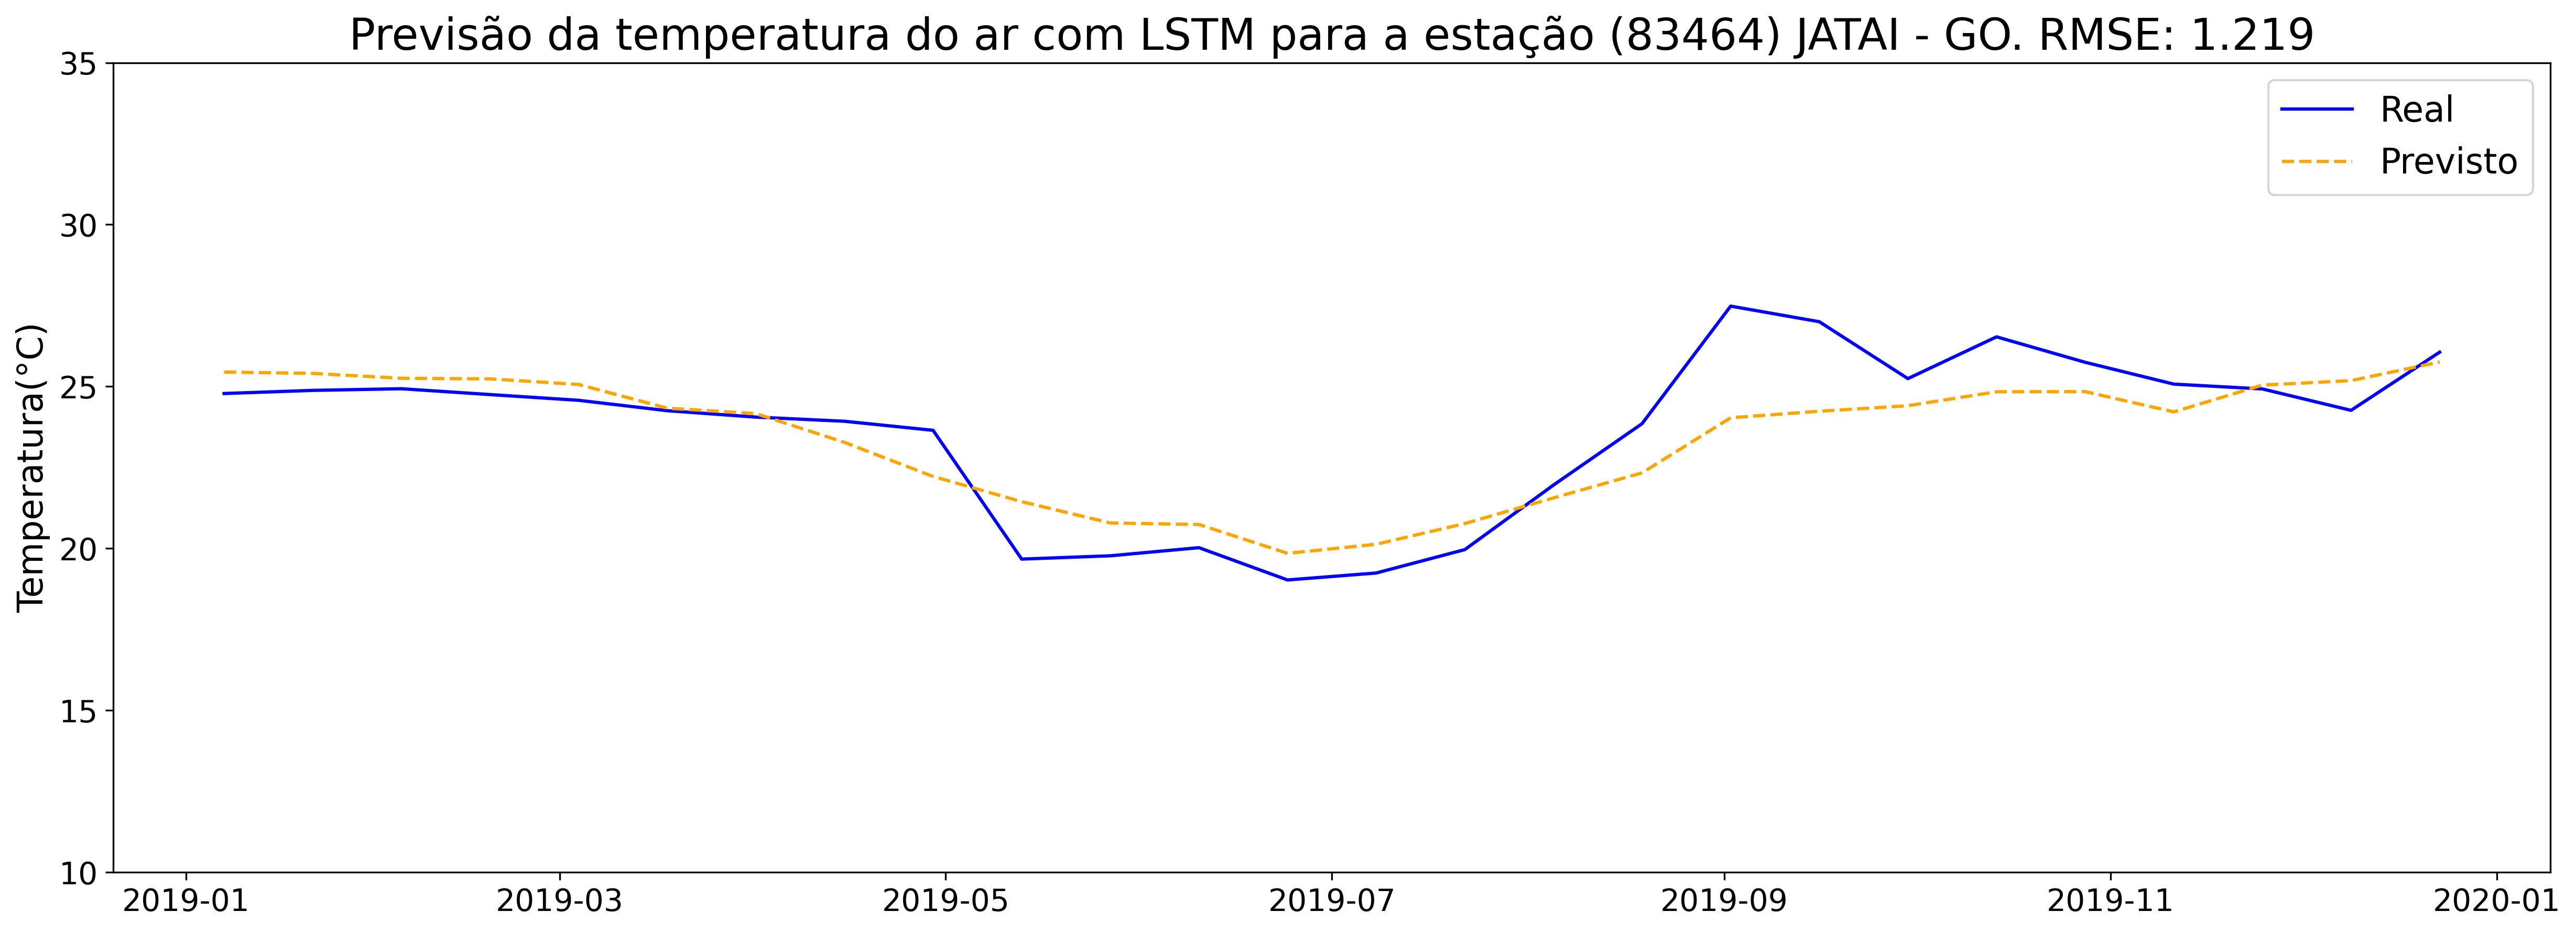
\includegraphics[scale=.30]{figuras/results/results_lstm_83464.png}}
\label{fig:results_lstm_83464}%
\end{figure}

\begin{figure}[H]%
\caption{Resultado das previsões da temperatura do ar para o ano de 2019 da estação meteorológica localizada no município de São Luiz Gonzaga, no estado do Rio Grande do Sul.}
\centering
\subfloat{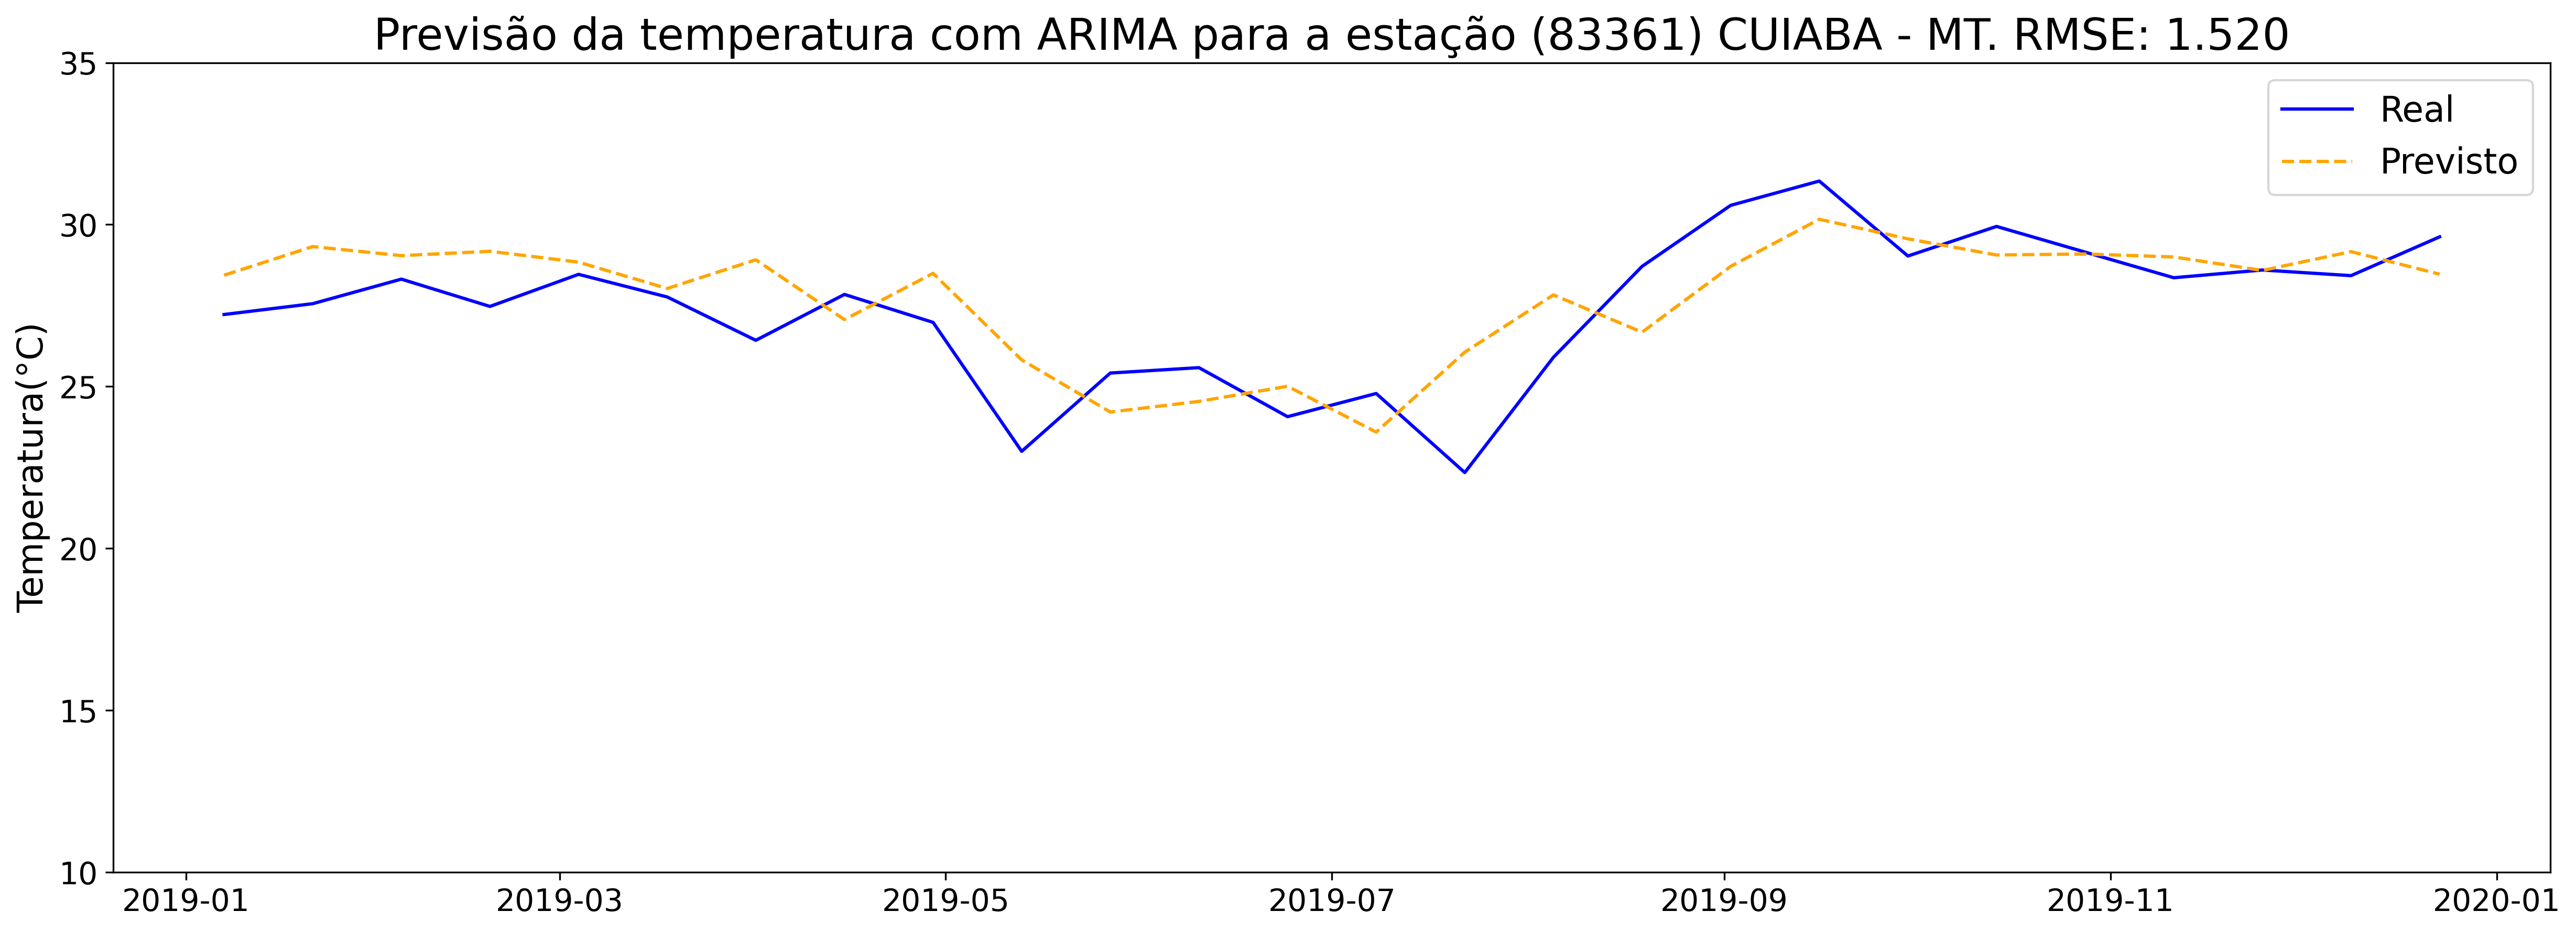
\includegraphics[scale=.30]{figuras/results/results_arima_83361.png}}
\qquad
\subfloat{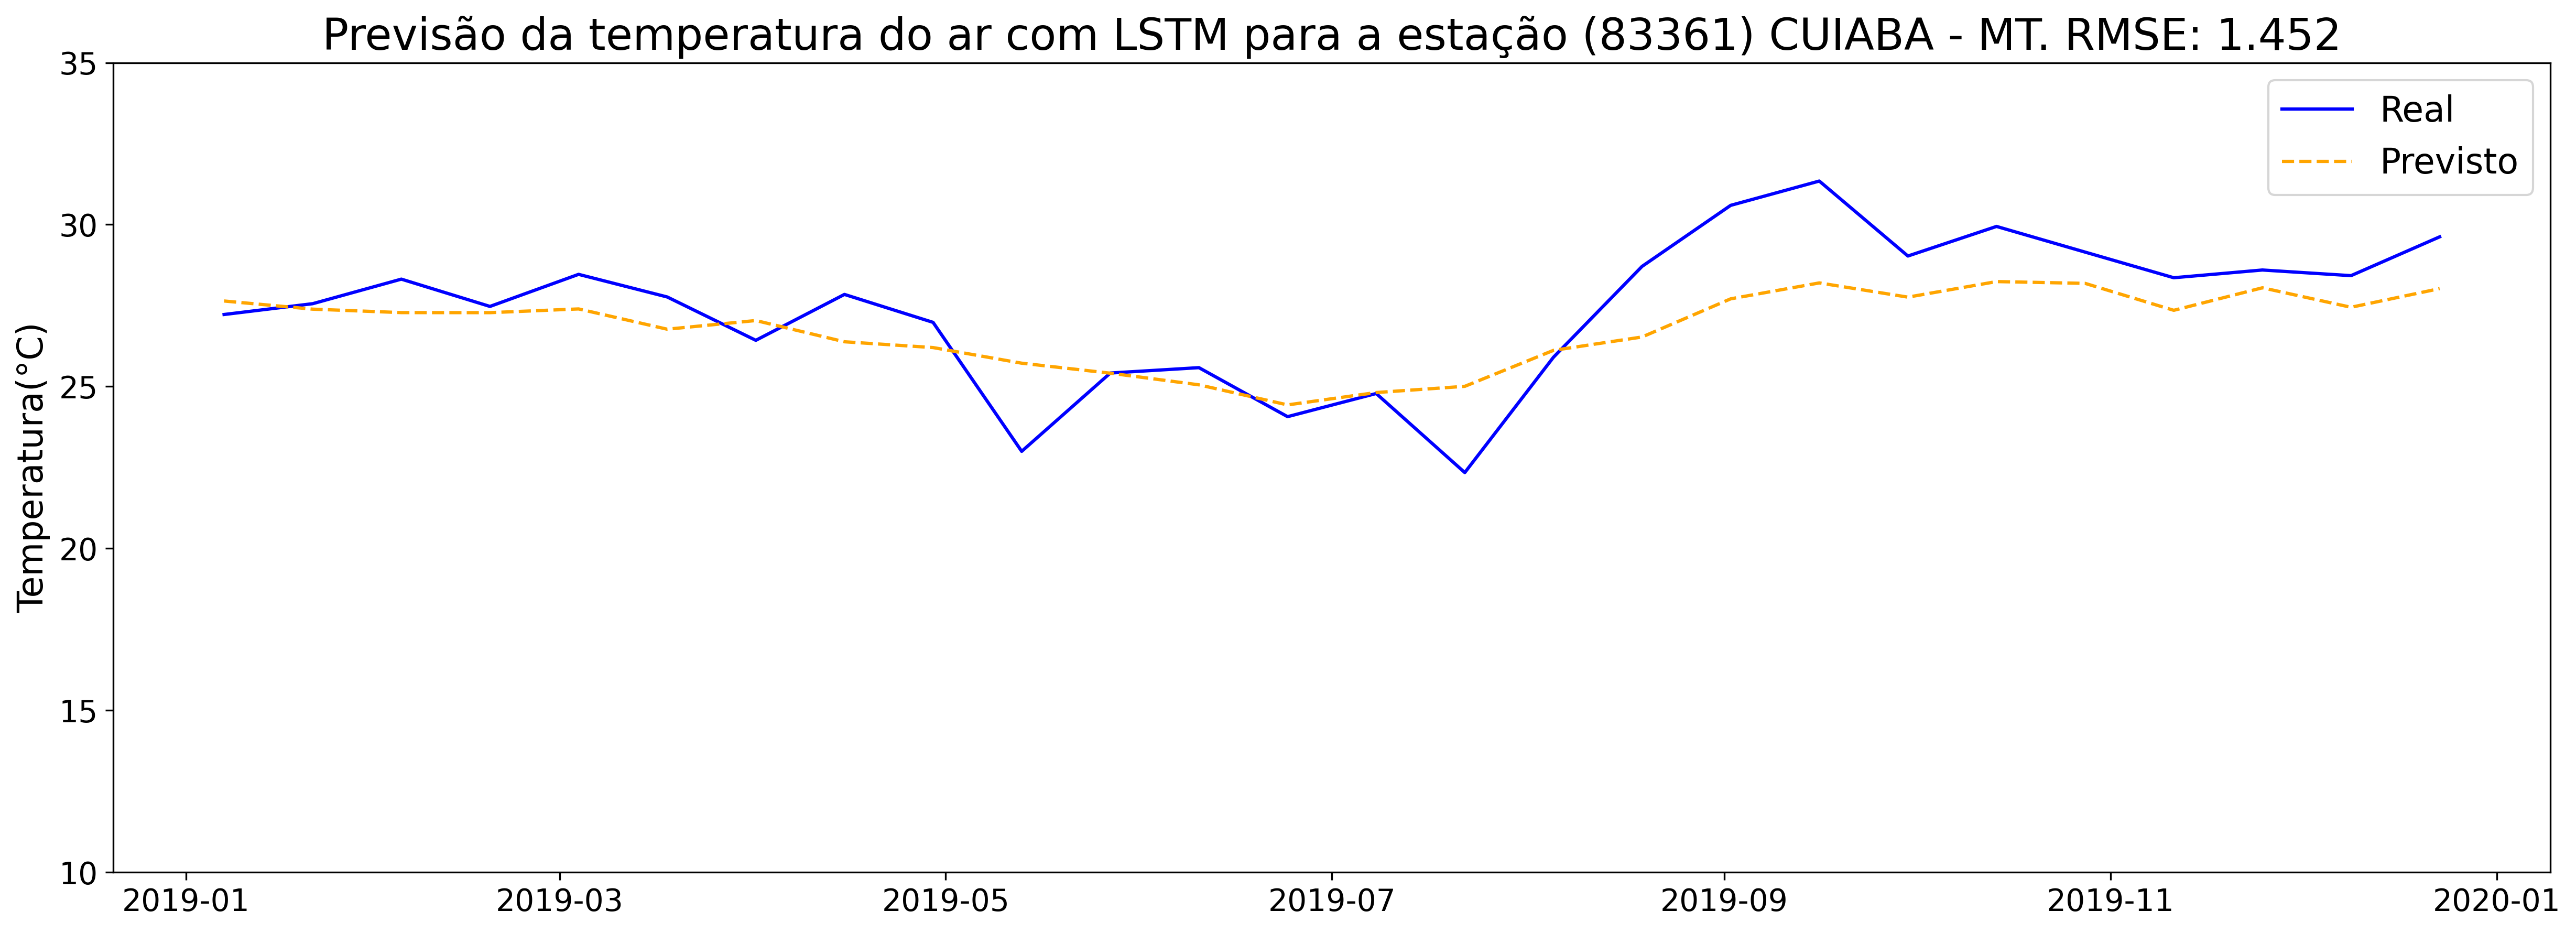
\includegraphics[scale=.30]{figuras/results/results_lstm_83361.png}}
\label{fig:results_lstm_83361}%
\end{figure}

\renewcommand{\cleardoublepage}{}
\renewcommand{\clearpage}{}
\vspace{5mm}